\documentclass{article}
\usepackage[utf8]{inputenc}
\usepackage{amsmath,amssymb}
\usepackage{graphicx}
\usepackage{booktabs}
\usepackage{hyperref}
\usepackage{xcolor}
\usepackage[margin=1in]{geometry}
\usepackage{caption}
\usepackage{subcaption}
\usepackage{enumitem}

\title{\textbf{Can a YouTube-Trained AI Brain Control a Robot?} \\[0.3em]
\large A Simplified Overview of Teach-by-Showing with Frozen Video Models}

\author{
Tung (Thomas) Vu Nguyen Nguyen \\
\texttt{thomas@beenex.ai}
}

\date{March 2026}

\begin{document}

\maketitle

% ============================================================
\begin{abstract}
What if a robot could learn to perform a task just by watching a single demonstration, using an AI ``brain'' that was trained on internet videos and never taught anything about robots? We test this idea using Meta's V-JEPA 2, a video understanding model with 325 million parameters. Without any retraining, we use it as the robot's visual system, add small prediction models on top, and let the robot plan its actions. Out of 7 simulated robot tasks, it works on 3 -- specifically the ones involving big, visible movements. Most surprisingly, one robot discovers a \emph{better} strategy than the one shown to it. The entire project cost less than \$30 in cloud GPU time.
\end{abstract}

% ============================================================
\section{What Problem Are We Solving?}

Teaching robots to see and act in the world is hard. The standard approach trains a custom vision system for each robot task from scratch. This is expensive: it needs millions of robot interactions or thousands of demonstrations, plus significant GPU compute.

We asked a simpler question: \textbf{Can we skip training the vision system entirely?}

Large AI models trained on internet video (like Meta's V-JEPA 2) already understand a lot about how the visual world works -- objects move, scenes change, physics applies. Maybe that's enough for a robot to work with.

\begin{figure}[h]
\centering
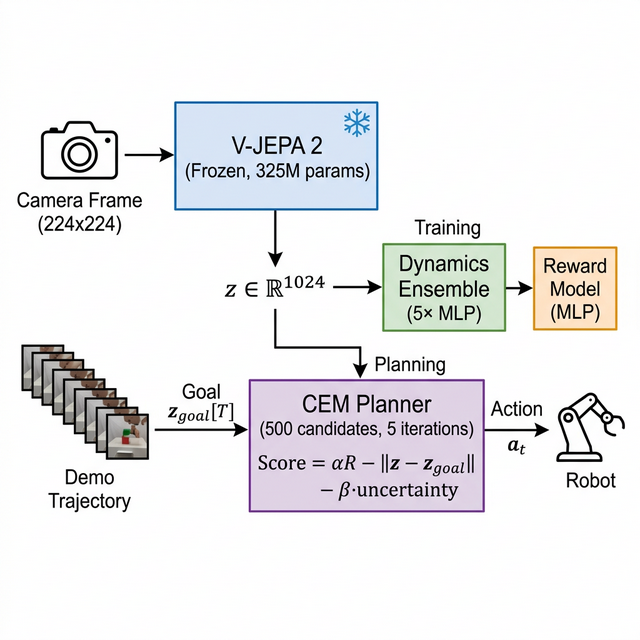
\includegraphics[width=0.85\linewidth]{figures/architecture.png}
\caption{\textbf{How our system works.} A camera frame goes through V-JEPA 2 (Meta's video AI, used as-is without any changes). Small prediction models learn the robot's physics. A planner tries 500 possible actions and picks the best one.}
\label{fig:arch}
\end{figure}

% ============================================================
\section{How Does It Work?}

Our system has four parts, each building on the previous one:

\subsection{Part 1: The Eyes (V-JEPA 2)}

V-JEPA 2 is an AI model that Meta trained by having it watch large amounts of internet video. It learned to predict what comes next in a video clip, which forced it to understand motion, object relationships, and scene dynamics.

We use V-JEPA 2 exactly as Meta released it -- no modifications. Each 224$\times$224 pixel camera frame goes in, and a compact summary of 1024 numbers comes out. These numbers capture the ``essence'' of the scene: where things are, how big they are, and what's happening.

\textbf{Does it actually understand?} To check, we trained simple linear classifiers on top of V-JEPA's output (Figure~\ref{fig:probe}). The results show that V-JEPA captures:
\begin{itemize}[nosep]
    \item Object position: R$^2$ = 0.86 (good)
    \item Object size: R$^2$ = 0.89 (very good)
    \item Object identity: 88.4\% accuracy (well above the 36\% random baseline)
\end{itemize}

\begin{figure}[h]
\centering
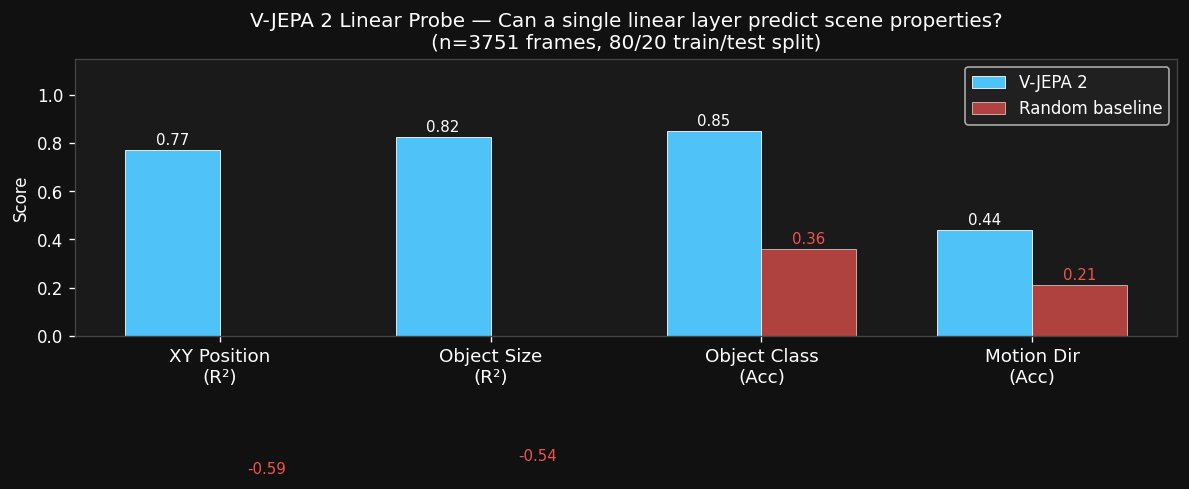
\includegraphics[width=0.75\linewidth]{figures/probe_summary.png}
\caption{\textbf{V-JEPA understands scene properties.} Using just a single linear equation on V-JEPA's output, we can predict object position, size, and identity far above chance. This model was never trained on robot data.}
\label{fig:probe}
\end{figure}

\subsection{Part 2: The Imagination (Dynamics Models)}

Next, we need the robot to be able to ``imagine'' what happens when it takes an action. If the robot moves its arm left, where does everything end up?

We train 5 small neural networks to answer this question. Each one takes the current scene summary + an action, and predicts the next scene summary. Having 5 models instead of 1 lets us measure confidence: if all 5 agree, the prediction is reliable; if they disagree, it's uncertain.

These models are tiny ($\sim$1.5 million parameters each, compared to V-JEPA's 325 million) and train in minutes. Figure~\ref{fig:dynamics} shows how quickly they learn.

\begin{figure}[h]
\centering
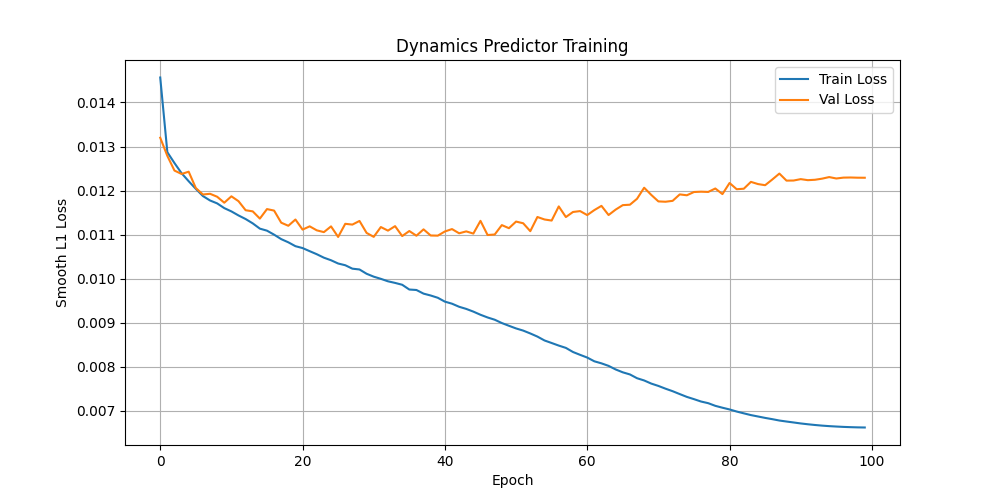
\includegraphics[width=0.55\linewidth]{figures/dynamics_loss.png}
\caption{\textbf{The ``imagination'' models learn fast.} Prediction error drops to near-zero within 100 training passes through the data.}
\label{fig:dynamics}
\end{figure}

\subsection{Part 3: The Demonstration (``Watch This'')}

To teach the robot a task, we simply \emph{show} it one demonstration. A policy (even a random one!) performs the task, and we record what V-JEPA sees at each moment. This creates a ``goal trajectory'' -- a sequence of scene summaries showing roughly what success looks like.

\begin{figure}[h]
\centering
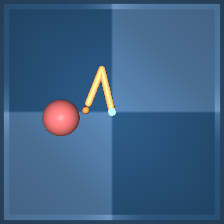
\includegraphics[width=0.22\linewidth]{figures/reacher_frame.png}
\caption{\textbf{Example task: Reacher.} The yellow arm must reach the red ball. We show the robot one demonstration, then ask it to do the same thing.}
\label{fig:reacher}
\end{figure}

\subsection{Part 4: The Planner (``What Should I Do Next?'')}

At each moment, the robot needs to decide what action to take. Here's how:

\begin{enumerate}[nosep]
    \item \textbf{Generate 500 random action plans} (each is a sequence of 8 actions).
    \item \textbf{Simulate each plan} using the imagination models: ``if I do these actions, where do I end up?''
    \item \textbf{Score each plan} based on three criteria:
    \begin{itemize}[nosep]
        \item Does it match the demonstration? (get close to the goal trajectory)
        \item Does the reward model predict high reward?
        \item Are the imagination models confident? (penalize uncertainty)
    \end{itemize}
    \item \textbf{Keep the best 50 plans}, generate new variations around them, and repeat 5 times.
    \item \textbf{Execute the first action} of the best plan, then replan from scratch.
\end{enumerate}

This approach (called the Cross-Entropy Method, or CEM) is robust because it doesn't commit to any single plan. It constantly evaluates many options and picks the best.

% ============================================================
\section{Results: What Worked, What Didn't}

We tested on 7 simulated robot tasks. Table~\ref{tab:results} shows the results.

\begin{table}[h]
\centering
\caption{\textbf{Results across all 7 tasks.} Reward is cumulative environment reward (higher = better). ``Shifted'' means the robot starts in a different position than the demonstration.}
\label{tab:results}
\begin{tabular}{lcccl}
\toprule
\textbf{Task} & \textbf{Same Start} & \textbf{Different Start} & \textbf{Verdict} \\
\midrule
Walker Walk & 13.5 & \textbf{20.1} & \textcolor{green!60!black}{\textbf{Works!}} \\
Cartpole Swingup & 14.4 & 14.3 & \textcolor{green!60!black}{\textbf{Works!}} \\
Reacher Easy & 6.1 & 8.5 & \textcolor{green!60!black}{\textbf{Works!}} \\
Cheetah Run & 1.7 & 1.4 & \textcolor{orange}{\textbf{Barely}} \\
Hopper Hop & 0.0 & 0.3 & \textcolor{red}{\textbf{Fails}} \\
Finger Spin & 0.0 & 0.0 & \textcolor{red}{\textbf{Fails}} \\
Point Mass & 0.0 & 1.4 & \textcolor{red}{\textbf{Fails}} \\
\bottomrule
\end{tabular}
\end{table}

\begin{figure}[h]
\centering
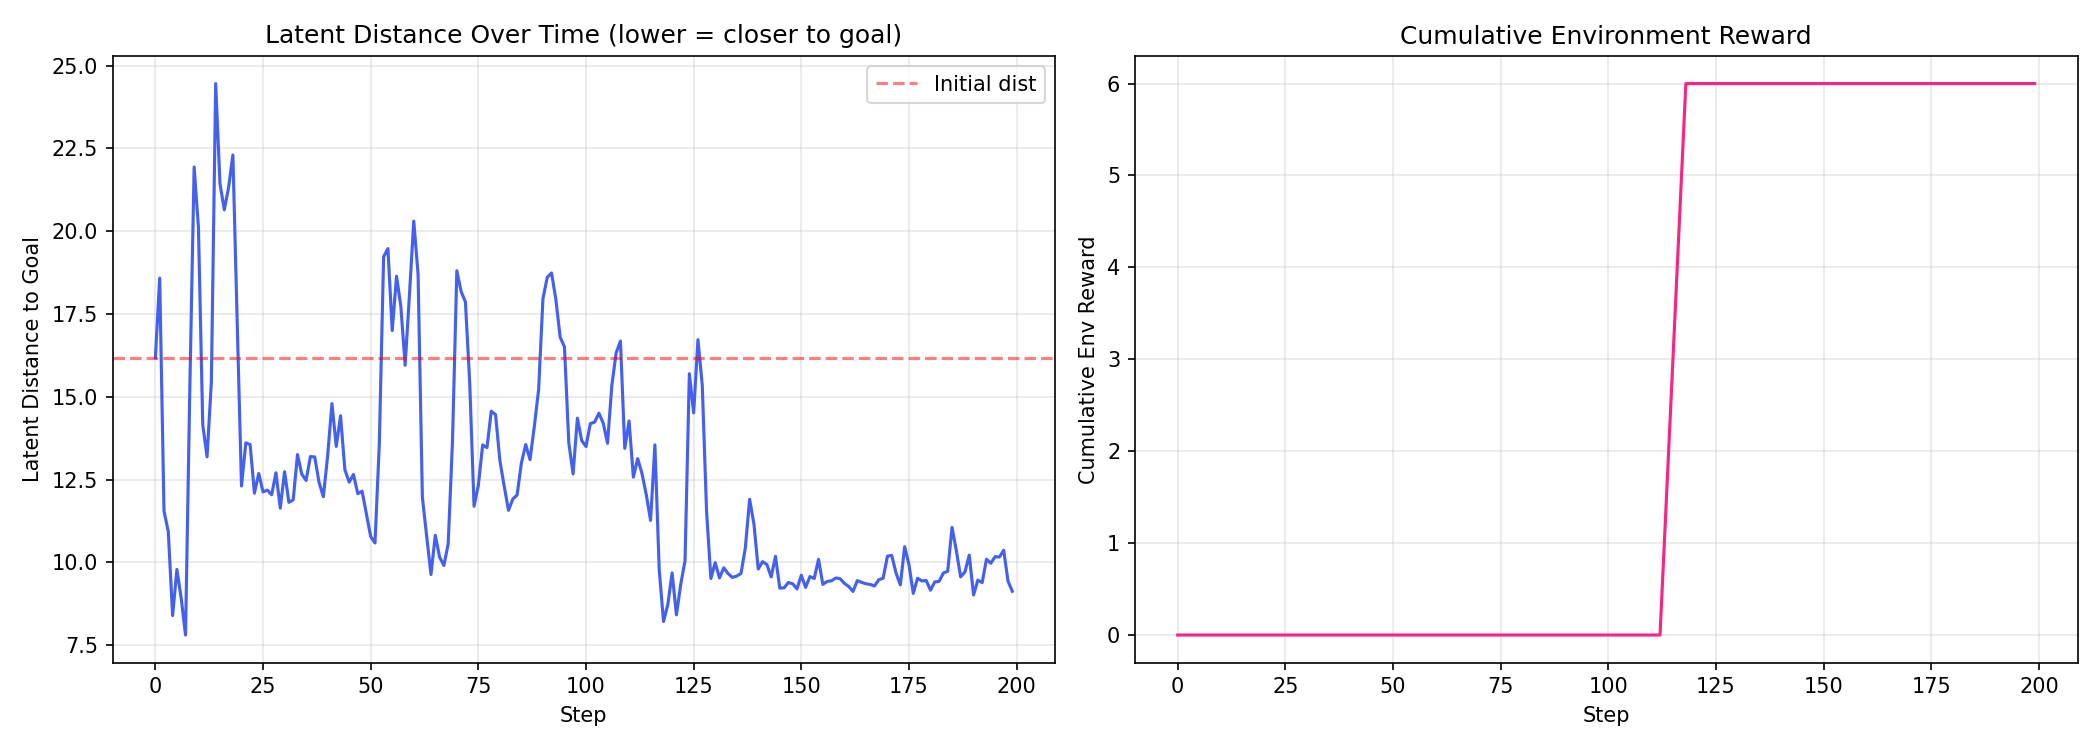
\includegraphics[width=0.85\linewidth]{figures/cem_metrics.png}
\caption{\textbf{Watching the planner work (Reacher task).} \emph{Left:} The robot's mental distance to the goal decreases over time as it follows the demonstration. \emph{Right:} Reward starts accumulating around step 100 when the arm reaches the target area.}
\label{fig:cem}
\end{figure}

\subsection{Two Surprising Discoveries}

\paragraph{Discovery 1: The walker beats its own demonstration.}
When the walking robot starts from a \emph{different} position than the demonstration, it actually performs \textbf{better} (20.1 vs 13.5). This means the robot isn't just blindly copying -- it genuinely understands the goal and finds more efficient strategies when starting fresh.

\paragraph{Discovery 2: The cartpole invents a skill it never saw.}
Our demonstration for the cartpole task came from a heuristic policy that scored near-zero (averaging $\sim$1.0 cumulative reward -- essentially failure). Yet the robot scores 14.4. It figured out how to swing up the pole despite never seeing it done successfully. The demonstration just pointed it in the right direction; the imagination models and planner did the rest.

\subsection{Why Did 4 Tasks Fail?}

The pattern is simple and revealing:

\begin{table}[h]
\centering
\caption{\textbf{Success depends on how visible the movements are.} V-JEPA learned from internet video, where motion is large-scale. It struggles with subtle, fine-grained changes.}
\label{tab:why}
\begin{tabular}{lll}
\toprule
\textbf{What the robot needs to see} & \textbf{Example} & \textbf{Does V-JEPA see it?} \\
\midrule
Large limb movements & Walker, Cartpole & \textcolor{green!60!black}{Yes -- similar to humans in video} \\
Visible arm motion & Reacher & \textcolor{green!60!black}{Yes -- colorful, distinct} \\
Subtle body deformation & Cheetah & \textcolor{orange}{Barely} \\
Tiny object rotation & Finger & \textcolor{red}{No -- too small on screen} \\
Small ball on plain background & Point Mass & \textcolor{red}{No -- not visually distinct} \\
\bottomrule
\end{tabular}
\end{table}

\textbf{The rule:} V-JEPA was trained on internet videos featuring people walking, objects moving, and scenes changing. It excels at detecting large, colorful motion. But it cannot reliably distinguish tiny positional differences or fine-grained rotations -- these simply aren't the type of visual changes it was trained on.

% ============================================================
\section{What Components Matter Most?}

We tested removing each piece to see what's actually important (Table~\ref{tab:ablation}).

\begin{table}[h]
\centering
\caption{\textbf{Ablation study:} removing components one at a time.}
\label{tab:ablation}
\begin{tabular}{lcc}
\toprule
\textbf{What we changed} & \textbf{Reacher Score} & \textbf{Effect} \\
\midrule
Full system (5 models + reward + uncertainty) & 18.0 & -- \\
Only 1 model instead of 5 & 4.4 & \textcolor{red}{4.1$\times$ worse} \\
Remove uncertainty penalty & 10.0 & \textcolor{orange}{1.8$\times$ worse} \\
Remove reward signal & 7.4 & \textcolor{orange}{Mixed (helps generalization)} \\
\bottomrule
\end{tabular}
\end{table}

\textbf{Key takeaways:}
\begin{itemize}[nosep]
    \item \textbf{Multiple models are essential} for complex tasks. Five models averaging their predictions are far more accurate than one.
    \item \textbf{The uncertainty penalty helps} but the effect is noisy and needs more experiments to confirm.
    \item \textbf{The reward signal is a double-edged sword.} It helps when the robot starts in the same position as the demo, but actually \emph{hurts} when starting from a different position. Pure goal-following generalizes better.
\end{itemize}

% ============================================================
\section{How Much Did This Cost?}

A distinctive feature of this approach is how cheap it is.

\begin{table}[h]
\centering
\caption{\textbf{Total project cost: \$29.99} on rented cloud GPUs (NVIDIA A100).}
\label{tab:cost}
\begin{tabular}{lr}
\toprule
\textbf{What we did} & \textbf{Cost} \\
\midrule
Collecting robot exploration data & \$3.30 \\
Robot control experiments & \$4.10 \\
Failed Dreamer experiment (learning from failure!) & \$1.60 \\
Training models for all 7 tasks & \$6.99 \\
Teaching-by-showing experiments & \$0.40 \\
Testing which components matter & \$1.00 \\
Overnight multi-task evaluation & \$6.40 \\
\midrule
\textbf{Total (including failures)} & \textbf{\$29.99} \\
\bottomrule
\end{tabular}
\end{table}

Because V-JEPA is frozen (never retrained), we only need to train tiny models. This makes the entire project accessible to anyone with \$30 and a rented GPU -- no expensive lab required.

% ============================================================
\section{What Does This Mean?}

\subsection{The Core Insight}

\begin{quote}
\emph{The quality of the AI's ``eyes'' determines the quality of its actions. When V-JEPA captures the right visual features, even simple planning works. When it doesn't, no amount of clever planning can compensate.}
\end{quote}

This has a practical implication: the bottleneck in using foundation models for robotics is not the planning algorithm, but the \emph{representation quality}. Future work should focus on improving what the model ``sees'' rather than making more sophisticated planners.

\subsection{Comparison to Other Approaches}

We initially tried Dreamer, a popular robot learning method that trains an actor-critic policy inside the model's imagination. It failed completely -- the robot learned to ``cheat'' by exploiting inaccuracies in the prediction models (taking actions that \emph{look} good to the model but do nothing useful). Our planner (CEM) avoids this by constantly trying many options instead of learning a single fixed policy.

\subsection{Limitations}

\begin{itemize}[nosep]
    \item Only 3 of 7 tasks work. The approach is limited to visually obvious tasks.
    \item Our demonstrations come from random policies. Expert demonstrations would likely improve results.
    \item The planner runs at about 7 decisions per second on an A100 GPU, which is too slow for some real-time applications.
    \item We tested only in simulation, not on real robots.
\end{itemize}

\subsection{What's Next?}

The most promising directions to extend this work:
\begin{enumerate}[nosep]
    \item \textbf{Fine-tune the last few layers} of V-JEPA on robot data, to help it see the subtle details it currently misses.
    \item \textbf{Use expert demonstrations} instead of random ones.
    \item \textbf{Combine vision with joint sensors} -- add direct measurements of the robot's arm angles and velocities.
    \item \textbf{Test on real robots}, where V-JEPA's internet video knowledge may provide even stronger benefits.
\end{enumerate}

% ============================================================
\section{Summary}

We showed that an AI video model (V-JEPA 2), trained entirely on internet video with no robot data, can serve as a robot's visual system. Without any retraining, it enables a robot to watch one demonstration and then copy it -- sometimes even improving on the original. The approach works when movements are big and visible, and fails when they are subtle. The entire project cost under \$30.

The key lesson: \textbf{representation quality is everything.} Get the ``eyes'' right, and simple planning suffices. Get them wrong, and nothing else can save you.

\end{document}
